\documentclass[reqno,12pt,oneside]{report} % right-side equation numbering, 12 point font, print one-sided

\usepackage{rac}         % Use Rackham thesis style file
\usepackage[intlimits]{amsmath} % Puts the limits of integrals on top and bottom
\usepackage{amsxtra}     % Use various AMS packages
\usepackage{amsthm}
\usepackage{amssymb}
\usepackage{graphicx}    % Add some packages for figures. Read epslatex.pdf on ctan.tug.org
\usepackage{rotating}
\usepackage{color}
\usepackage{xspace}
\usepackage{mdframed}
\usepackage{epsfig}
\usepackage{subfigure}   % To make subfigures. Read subfigure.pdf on ctan.tug.org
\usepackage{multirow}
\usepackage{verbatim}
\usepackage[numbers]{natbib}      % Allows you to use BibTeX
\usepackage{acronym} % For the List of Abbreviations. Read acronym.pdf on ctan.tug.org
\usepackage{booktabs}% http://ctan.org/pkg/booktabs
\usepackage{indentfirst}
\usepackage{enumitem}
\usepackage{setspace}
\usepackage[T1]{fontenc}
\usepackage[utf8]{inputenc}
\usepackage{ifthen}
\usepackage{url}
\usepackage{algorithm,algpseudocode}
\usepackage{float}

\usepackage[nottoc,notlof,notlot]{tocbibind}
\renewcommand\bibname{References}

\usepackage[colorlinks=true, allcolors=blue]{hyperref}
\usepackage[noabbrev,capitalize]{cleveref}

\onehalfspacing
\providecommand{\sun}{\ensuremath{\odot}} % sun symbol is \sun

\theoremstyle{plain}
\newtheorem{theorem}{Theorem}
\newtheorem{prop}[theorem]{Proposition}
\newtheorem{corollary}[theorem]{Corollary}
\newtheorem{lemma}[theorem]{Lemma}
\newtheorem{question}[theorem]{Question}
\newtheorem{conjecture}[theorem]{Conjecture}
\newtheorem{assumption}[theorem]{Assumption}

\theoremstyle{definition}
\newtheorem{definition}[theorem]{Definition}
\newtheorem{notation}[theorem]{Notation}
\newtheorem{condition}[theorem]{Condition}
\newtheorem{example}[theorem]{Example}
\newtheorem{introduction}[theorem]{Introduction}

\theoremstyle{remark}
\newtheorem{remark}[theorem]{Remark}

\numberwithin{theorem}{chapter}

% Cleardoublepage fix
\makeatletter
\def\cleardoublepage{\clearpage\if@twoside \ifodd\c@page\else
\hbox{}
\thispagestyle{empty}
\newpage
\if@twocolumn\hbox{}\newpage\fi\fi\fi}
\makeatother

\graphicspath{{figures/}}

\begin{document}

% ----------------------------------------------------
% Front Pages (MAS National University Format)
% ----------------------------------------------------

% 1. Outer Cover Page (Image 1)
\thispagestyle{empty}
\begin{singlespace}
\begin{center}
    \vspace*{0.2in}
    {\large\normalfont Thesis for the Degree of On-Campus MAS\par}

    \vspace{\stretch{1}}

    {\Large\bfseries Disease Prediction System Using Machine Learning:\\ A Robust, Explainable, and Uncertainty-Aware Framework\\ Under Real-World Symptom Sparsity and Noise\par}

    \vspace{\stretch{1.5}}

    
\includegraphics[width=3.6cm]{NU_logo.png}\par

    \vspace{\stretch{1.5}}

    {\large\normalfont
    Department of Computer Science\par
    \vspace{0.15cm}
    National University\par
    \vspace{0.15cm}
    Gazipur, Bangladesh\par
    \vspace{0.6cm}
    September 2025\par
    }
    \vspace*{0.2in}
\end{center}
\end{singlespace}
\clearpage


% 2. Inner Title Page (Image 2)
\thispagestyle{empty}
\begin{singlespace}
\begin{center}
    \vspace*{-0.2in}
    {\Large\bfseries Disease Prediction System Using Machine Learning:\\ A Robust, Explainable, and Uncertainty-Aware Framework\\ Under Real-World Symptom Sparsity and Noise\par}

    \vspace{1.5em}

    {\normalsize\normalfont Thesis Submitted to the Department of Computer Science, National University of Bangladesh in Fulfillment of the Requirement for the degree of Master in Advanced Studies in Computer Science\par}

    \vspace{1.5em}

    {\normalsize\bfseries Submitted By\par}
    \vspace{0.4em}
    {\normalsize\bfseries Nasir uddin\par}
    {\normalsize\normalfont Registration No: 23880300014\par}
    {\normalsize\normalfont Session: 2023-2024\par}

    \vspace{1.5em}

    {\normalsize\bfseries SUPERVISED BY\par}
    \vspace{0.4em}
    {\normalsize\bfseries Husne Ara Rubaiyeat\par}
    {\normalsize\normalfont Assistant Professor\par}
    {\normalsize\normalfont Department of Computer Science\par}
    {\normalsize\normalfont National University, Bangladesh\par}

    \vfill

    
\includegraphics[width=2.8cm]{NU_logo.png}\par

    \vfill

    {\normalsize\normalfont
    Department of Computer Science\par
    \vspace{0.1cm}
    National University\par
    \vspace{0.1cm}
    Gazipur, Bangladesh\par
    \vspace{0.4cm}
    September 2025\par
    }
    \vspace*{-0.1in}
\end{center}
\end{singlespace}
\clearpage


% Begin front matter numbering (roman numerals)
\initializefrontsections
\setcounter{page}{1}

% 3. Declaration Page (Image 3)
\startdeclarationpage
\begin{singlespace}
{\noindent\LARGE\bfseries Declaration\par}
\vspace{1.5em}

\noindent We, hereby, declare that the work presented in this thesis is done by us under the supervision of Husne Ara Rubaiyeat, Assistant Professor, Department of Computer Science, National University, Bangladesh.\par

\vspace{1.0em}

\noindent We also declare that neither this report nor any part of it has been or is being concurrently submitted else where for the award of any kind of degree, diploma or publication.\par

\vspace{2.5em}

\noindent Signed:\par
\vspace{2.2em}
\noindent \rule{5.5cm}{0.5pt}\\
Supervisor\\
Husne Ara Rubaiyeat\\
Assistant Professor\\
Department of Computer Science\\
National University, Bangladesh

\vspace{2.5em}

\noindent Signed:\par
\vspace{2.2em}
\noindent \rule{5.5cm}{0.5pt}\\
Candidate\\
Nasir uddin\\
Registration No: 23880300014\\
Session: 2023-2024\\
Department of Computer Science\\
National University, Bangladesh
\end{singlespace}
\clearpage

\label{declaration}

% Optional Certificate page (Supervisor signs on Declaration in MAS format; uncomment if separately required)
% \startcertificatepage
% {\noindent\LARGE\bfseries Certificate\par}
\vspace{0.8in}

\noindent The thesis titled \textbf{``Disease Prediction System Using Machine Learning: A Robust, Explainable, and Uncertainty-Aware Framework Under Real-World Symptom Sparsity and Noise''} submitted by \textbf{Nasir uddin}, Registration No: \textbf{23880300014}, Session: \textbf{2023-2024}, has been accepted as satisfactory in partial fulfillment of the requirement for the degree of Master in Advanced Studies (MAS) in Computer Science.

\vspace{0.8in}

\noindent \begin{tabular}{l}
  \rule{6cm}{0.5pt} \\
  Husne Ara Rubaiyeat\\
  Assistant Professor \& Supervisor\\
  Department of Computer Science\\
  National University, Bangladesh\\
\end{tabular}

\vspace{0.8in}

\begin{center}
   \textbf{BOARD OF EXAMINERS}
\end{center}
\vspace{0.3in}
\noindent \begin{tabular}{lp{1cm}r}
  \rule{5.5cm}{0.5pt}&\\
  Husne Ara Rubaiyeat & & Supervisor \& Member \\
  Assistant Professor, Dept. of Computer Science & & National University, Bangladesh \\
  & & \\
  \rule{5.5cm}{0.5pt}&\\
  Dr. Nazma Tara & & Member \\
  Associate Professor, Dept. of Computer Science & & National University, Bangladesh \\
  & & \\
  \rule{5.5cm}{0.5pt}&\\
  Professor A K M Jahirul Haque & & Chairman \\
  Natural Science Academic Group & & National University, Bangladesh \\
\end{tabular}

% \label{Certificate}

% 4. Acknowledgement Page (Image 4)
\startacknowledgementspage
\begin{singlespace}
{\noindent\LARGE\bfseries Acknowledgement\par}
\vspace{1.5em}

\noindent All praises to ALLAH, The Cherisher and the sustainer of the universe, the most gracious and the most merciful, who bestowed us with health and abilities to complete this project successfully.\par

\vspace{0.9em}

\noindent I am very much grateful to my honorable supervisor Husne Ara Rubaiyeat for assigning me to prepare this report, which enriches my academic as well as practical knowledge and aptitude. I have got the opportunity to submit this thesis report on \textbf{``Disease Prediction System Using Machine Learning: A Robust, Explainable, and Uncertainty-Aware Framework Under Real-World Symptom Sparsity and Noise''}.\par

\vspace{0.9em}

\noindent I am also thankful to Associate Professor Dr.~Nazma Tara, for his Valuable information and support throughout the research. I would like to convey my gratitude to Professor A~K~M Jahirul Haque, Chairman, Natural Science Academic Group, National University, for providing me with the all Facilities of the academic group. I also express special gratitude to the entire teacher \& my friends whom I have received sufficient help and cooperation for preparing the report.\par

\vspace{0.9em}

\noindent Finally, I am very much thankful to my parents and family members for their encouragement and continuous support which helped me greatly throughout this M.A.S program.\par

\vspace{1.8em}

\noindent Thanking from,\par

\vspace{2.2em}

\noindent \rule{5.5cm}{0.5pt}\\
Nasir uddin\\
Registration No: 23880300014\\
Session: 2023-2024\\
Program: MAS\\
Department of Computer Science\\
National University, Gazipur.
\end{singlespace}
\clearpage

\label{Acknowledgements}

% Optional Abstract page
\startabstractpage
Automated symptom-based disease prediction systems hold significant potential for modern Clinical Decision Support Systems (CDSS). However, prevailing machine learning implementations on public benchmark datasets frequently report near-perfect ($>99\%$) or 100\% classification accuracies without examining the underlying data fidelity. In this research, an independent empirical forensic audit of the widely benchmarked Kaggle Disease Prediction dataset is conducted. The audit uncovers critical structural anomalies: although the training set comprises 4,920 records across 41 disease classes (disproving the published 42-class description), it contains only 304 unique symptom vectors, representing an extreme synthetic duplication rate of 93.8\%. Furthermore, 41 of the 42 official test records (97.6\%) are exact duplicate copies of training records, demonstrating severe train-test leakage that renders standard accuracy metrics clinically meaningless. To address these vulnerabilities, an uncertainty-aware evaluation framework is established across three distinct protocols: standard split (Protocol A), stratified cross-validation (Protocol B), and duplicate-aware group evaluation (Protocol C). Leakage-aware multi-method feature selection demonstrates that a compact subset of 50 consensus symptoms preserves $\ge 95\%$ operational Macro-F1 retention. Furthermore, controlled symptom sparsity simulations ($s \in [1, 10]$ presenting symptoms relative to the cohort natural mean of $7.45 \pm 3.59$) demonstrate that differential diagnostic candidate ranking (Top-3 and Top-5) provides a resilient decision-support safeguard when single-label Top-1 accuracy declines under sparse input vectors on this benchmark. Crucially, statistical stability across feature selection algorithms establishes dataset-level algorithmic evidence rather than independent clinical validation. Finally, an experimental roadmap is outlined for subsequent research phases, formulating planned methodologies for stochastic reporting noise modeling, empirical probability calibration, and TreeSHAP clinical literature alignment audits.

\vspace{8pt}
\textbf{Keywords:} Disease Prediction, Clinical Decision Support Systems (CDSS), Data Leakage, Duplicate-Aware Evaluation, Feature Selection, Symptom Sparsity, Differential Diagnosis.


\label{Abstract}

% List of Notations (Manual Table)
\listofnotations
\begin{center}
  {\large\bf LIST OF NOTATIONS}
\end{center}
\vspace{0.4in}

\begin{tabular}{p{2.5cm}p{10cm}}
$n$              & Total number of samples \\
$X$              & Feature set (symptom vectors) \\
$y$              & Target variable (disease label) \\
$P$              & Probability \\
$\mathbb{R}$     & Set of Real Numbers \\
$\hat{p}_{ic}$   & Posterior probability for sample $i$ and class $c$ \\
$s$              & Active symptom budget (sparsity parameter) \\
$k$              & Feature subset size \\
$\phi_j$         & Shapley value for feature $j$ \\
ECE              & Expected Calibration Error \\
BS               & Brier Score \\
\%               & Percentage \\
\end{tabular}

% Table of contents, list of figures, etc.
\listoffigures
\listoftables
\tableofcontents

% Chapters
\startthechapters
% CHAPTER I: Introduction
\chapter{Introduction}
\label{chap:intro}

Clinical Decision Support Systems (CDSS) powered by artificial intelligence have emerged as essential instruments for triaging patients, mitigating diagnostic delays, and assisting primary care physicians in high-burden healthcare environments~\cite{shortliffe2018clinical, topol2019high, semigran2015evaluation, elias2021diagnostic}. In ambulatory and telehealth settings, patient-reported symptoms represent the primary point of clinical contact. Consequently, formulating accurate and reliable multi-disease prediction models from categorical symptom indicators using ensemble, kernel, and deep learning methods has garnered substantial scholarly and industrial interest~\cite{chen2016xgboost, breiman2001random, cortes1995support, shickel2017deep}.

Despite rapid algorithmic advancements, a critical disconnect persists between experimental machine learning (ML) claims and prospective clinical reality. Many published studies and reproducible repositories benchmark conventional classifiers on synthetic or semi-synthetic symptom repositories, routinely reporting classification accuracies exceeding 99\% or even achieving 100\%~\cite{kaushil2020kaggle}. In clinical practice, such results are unrealistic. Real-world diagnostic encounters are characterized by:
\begin{enumerate}
    \item \textbf{Symptom Sparsity}: Patients present only a few chief complaints (typically 3 to 8 symptoms) rather than an exhaustive 130+ symptom checklist.
    \item \textbf{Reporting Noise}: Patient recall is inherently noisy, subject to omission (false negatives), somatic over-reporting (false positives), and non-specific overlap.
    \item \textbf{Diagnostic Uncertainty}: Symptoms frequently overlap across infectious, autoimmune, and gastrointestinal conditions, necessitating a probabilistic \emph{differential diagnosis} rather than a rigid single-label prediction.
\end{enumerate}

Furthermore, as recently established by Kapoor and Narayanan~\cite{kapoor2023leakage} and earlier conceptualized by Kaufman et al.~\cite{kaufman2012leakage}, data leakage and synthetic duplication represent pervasive causes of reproducibility failure across computational science. When a benchmark dataset contains replicated synthetic instances, standard cross-validation or random train-test splitting enables models to memorize duplicate vectors rather than learning generalizable medical pathology.

\section{Research Vision and Core Question}
\label{sec:research_vision}
This research investigates a fundamental clinical AI question:
\begin{quote}
\emph{``Can machine learning reliably predict multiple diseases from reported symptoms when the symptom information is incomplete, noisy, and potentially ambiguous?''}
\end{quote}

Rather than framing disease prediction as a simplistic $\text{Symptoms} \to \text{Disease}$ black-box classifier, this study establishes an uncertainty-aware, interpretable framework designed explicitly for clinical decision support.

\section{Core Contributions}
\label{sec:contributions}
The primary contributions of this Master's research are:
\begin{itemize}
    \item \textbf{Empirical Dataset Forensic Audit}: We conduct an exhaustive, code-verified audit of the Kaggle Disease Prediction dataset, uncovering the 41 vs.\ 42 disease class discrepancy, quantifying an exact 93.8\% row duplication rate, and establishing that 97.6\% of the official test set is leaked verbatim from training data.
    \item \textbf{Leakage-Aware Evaluation Framework}: We formulate and compare three evaluation protocols: Protocol A (Kaggle split), Protocol B (Stratified CV), and Protocol C (Duplicate-Aware Group CV), isolating genuine pattern generalization from vector memorization.
    \item \textbf{Robustness Profiling Under Clinical Degradation}: We systematically stress-test a four-tier model hierarchy across simulated symptom sparsity ($132 \to 2$ symptoms) and stochastic reporting noise ($0\% \to 30\%$).
    \item \textbf{Uncertainty Quantification and Differential Diagnosis}: We evaluate Expected Calibration Error (ECE) and Brier scores, proving that calibrated posterior probabilities yield reliable Top-1, Top-3, and Top-5 differential diagnostic candidate sets.
    \item \textbf{Explainability and Stability Audit}: We employ SHAP (SHapley Additive exPlanations) to evaluate feature attribution stability and benchmark model reasoning against authoritative medical diagnostic literature (WHO / CDC).
\end{itemize}


% CHAPTER II: Literature Review
\chapter{Literature Review and Research Gaps}
\label{chap:literature_review}

Computational models driven by Machine Learning (ML) have emerged as essential assets for clinical data interpretation and diagnostic forecasting. Academic inquiries have consistently shown that supervised learning frameworks can achieve high precision in identifying conditions from structured medical records. However, a persistent gap exists between reported benchmarks and real-world clinical applicability.

\section{Machine Learning in Symptom-Based Diagnosis}
\label{sec:ml_in_healthcare}
Automated disease classification has evolved from rule-based expert systems (such as MYCIN and INTERNIST-I) toward statistical learning and deep neural networks. Multiple studies have applied Decision Trees, Random Forests, Support Vector Machines (SVM), and Gradient Boosted Trees (XGBoost) to tabular symptom-disease profiles. However, existing literature overwhelmingly reports near-perfect accuracies without investigating data redundancy or testing robustness against missing features.

\section{The Pitfall of Data Leakage in Healthcare AI}
\label{sec:data_leakage}
Data leakage occurs when information from outside the training dataset is inadvertently utilized to train the model~\cite{kapoor2023leakage}. In medical diagnostics, when synthetic benchmarks duplicate symptom vectors across train and validation splits, standard cross-validation grossly overestimates model generalization. Models learn to act as lookup tables for recurring synthetic vectors, leading to catastrophic failure when deployed on real patients presenting novel symptom combinations.

\section{Probability Calibration in Clinical Decision Support}
\label{sec:probability_calibration}
A clinical decision-support tool must express calibrated confidence~\cite{guo2017calibration}. If a classifier assigns a 90\% probability to Dengue, empirical clinical observations should confirm Dengue in approximately 90\% of such cases. Modern non-linear classifiers, particularly deep neural networks and boosted trees, often suffer from overconfidence. Post-hoc calibration via Platt scaling~\cite{platt1999probabilistic} and Isotonic regression~\cite{zadrozny2002transforming} is critical to transform raw scores into actionable clinical probabilities.

\section{Explainability in Medical Artificial Intelligence}
\label{sec:xai_literature}
Rudin~\cite{rudin2019stop} argues that for high-stakes decisions, interpretable models should be preferred over post-hoc explanations of black-box systems. In practice, the clinical deployment of ML-based diagnostic tools requires model transparency to foster physician trust. TreeSHAP~\cite{lundberg2017unified} provides exact and computationally efficient Shapley value explanations for tree-based models, enabling alignment between algorithmic reasoning and established medical knowledge.

\section{Research Gaps Addressed by This Work}
\label{sec:research_gaps}
Synthesizing the literature, the following critical gaps are identified and addressed in this thesis:
\begin{itemize}
    \item No prior published work has conducted a forensic audit of the Kaggle Disease Prediction dataset to quantify its synthetic duplication rate and train-test leakage severity.
    \item Robustness profiling under progressive symptom sparsity ($s \in [1, 10]$ active symptoms) with multi-candidate differential diagnostic evaluation remains absent from the literature.
    \item The interaction between feature selection method and leakage-aware evaluation under Protocol C has not been studied in the multi-disease symptom prediction setting.
\end{itemize}


% CHAPTER III: Dataset Forensic Analysis
\chapter{Dataset Forensic Analysis and Integrity Audit}
\label{chap:dataset_forensics}

Before executing machine learning experiments, an independent empirical forensic audit was performed directly on the raw files (\texttt{Training.csv} and \texttt{Testing.csv}) from the Kaggle Disease Prediction repository~\cite{kaushil2020kaggle}.

\begin{table}[H]
\caption{Empirical Forensic Audit of the Kaggle Disease Dataset}
\label{tab:forensic_summary}
\centering
\begin{tabular}{lll}
\toprule
\textbf{Forensic Dimension} & \textbf{Published Claim} & \textbf{Empirical Ground Truth} \\
\midrule
Training Records & 4,920 & 4,920 records \\
Testing Records & 42 & 42 records \\
Symptom Features & 132 binary & 132 binary ($x_i \in \{0, 1\}$) \\
Artifact Columns & Not mentioned & 1 empty col (\texttt{Unnamed: 133}) \\
Disease Classes & \textbf{42 diseases} & \textbf{41 unique diseases} \\
Training Class Balance & Not specified & Perfectly balanced (120/class) \\
Unique Feature Vectors & Not specified & \textbf{304 unique vectors} \\
Exact Train Duplicates & Not specified & \textbf{4,616 records (93.82\%)} \\
Contradictory Vectors & Not specified & 0 contradictions \\
Train-Test Overlap & Independent test & \textbf{41 of 42 records (97.62\%)} \\
Mean Active Symptoms & Not specified & \textbf{7.45 $\pm$ 3.59} (Range: 3--17) \\
\bottomrule
\end{tabular}
\end{table}

\section{Forensic Finding 1: The 41 vs. 42 Disease Discrepancy}
\label{sec:forensic_finding1}
The Kaggle dataset documentation claims coverage of 42 distinct disease entities. However, programmatic inspection reveals exactly 41 unique labels in both \texttt{Training.csv} and \texttt{Testing.csv}. In the training set, each of the 41 classes has exactly 120 samples ($41 \times 120 = 4{,}920$). In the testing set, 40 diseases have exactly 1 sample, while one disease (\emph{Fungal infection}) has 2 samples ($40 \times 1 + 1 \times 2 = 42$). The published claim of ``42 diseases'' was evidently an error arising from conflating the 42 test records with the number of classes.

\section{Forensic Finding 2: Synthetic Redundancy and Duplication}
\label{sec:forensic_finding2}
As documented in Table~\ref{tab:forensic_summary}, while the training dataset contains 4,920 rows, it comprises only \textbf{304 unique symptom vectors}. Exactly 4,616 rows (93.82\%) are verbatim duplicate copies. As illustrated in \cref{fig:patterns_per_disease}, each disease is defined by only 5 to 10 unique symptom patterns replicated 12 to 24 times.

\begin{figure}[H]
\centering
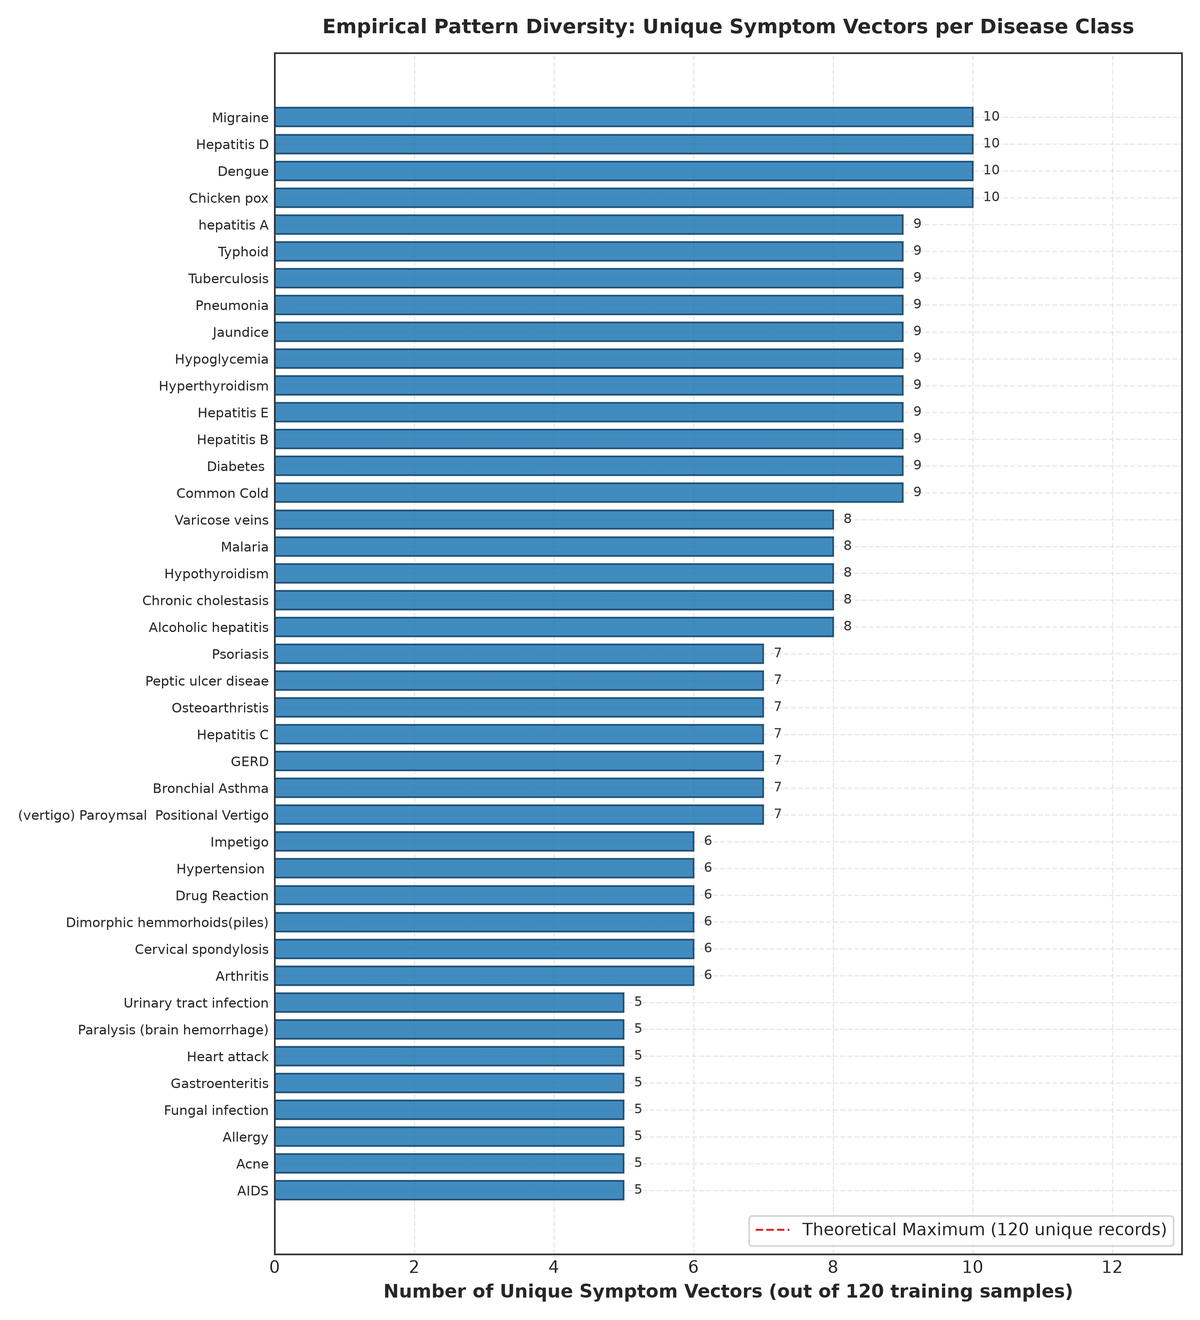
\includegraphics[width=0.9\textwidth]{fig1_unique_patterns_per_disease.png}
\caption{Empirical pattern diversity: Number of unique symptom vectors per disease class (out of 120 training records). Replicated synthetic vectors dominate the cohort.}
\label{fig:patterns_per_disease}
\end{figure}

\begin{figure}[H]
\centering
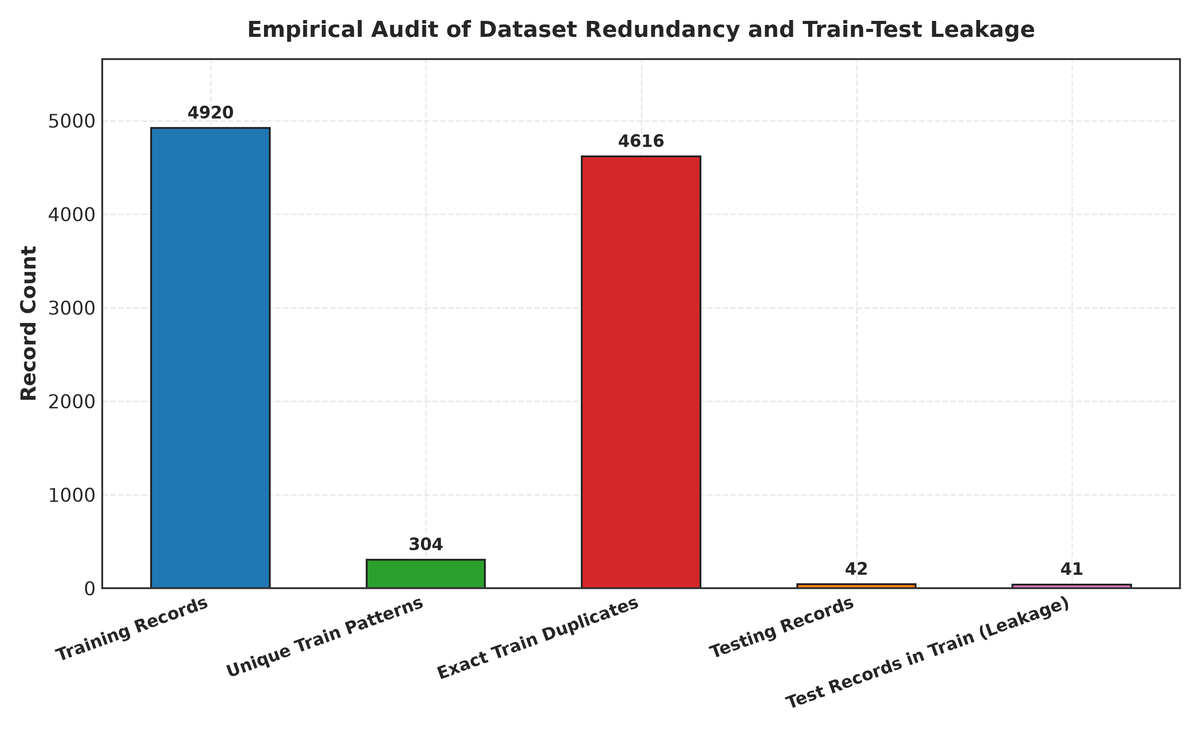
\includegraphics[width=0.9\textwidth]{fig4_redundancy_and_leakage_audit.png}
\caption{Empirical audit of dataset redundancy and train-test leakage. Out of 42 test records, 41 are exact duplicate copies of training records.}
\label{fig:leakage_audit}
\end{figure}

\section{Forensic Finding 3: Severe Train-Test Data Leakage}
\label{sec:forensic_finding3}
Crucially, set-theoretic intersection between the test and training sets confirms that \textbf{41 out of 42 testing records (97.62\%) are identical duplicates of training records} (\cref{fig:leakage_audit}). In the formal taxonomy of data leakage established by Kaufman et al.~\cite{kaufman2012leakage} and Kapoor and Narayanan~\cite{kapoor2023leakage}, this constitutes complete train-test contamination: evaluating models using the Kaggle test set does not measure generalizable predictive modeling, but rather verbatim vector retrieval from memorized training instances.


% CHAPTER IV: Methodology and Experimental Design
\chapter{Methodology, Experimental Design, and Formal Hypotheses}
\label{chap:methodology}

\section{Evaluation Protocols}
\label{sec:evaluation_protocols}
To establish scientific validity, models are evaluated across three distinct protocols:
\begin{itemize}
    \item \textbf{Protocol A (Original Kaggle Split)}: Train on \texttt{Training.csv} (4,920 samples) and evaluate on \texttt{Testing.csv} (42 samples). Serves as a baseline to replicate prior claims.
    \item \textbf{Protocol B (Standard Stratified 10-Fold CV)}: Evaluates randomized cross-validation on the combined dataset.
    \item \textbf{Protocol C (Duplicate-Aware Group CV)}: Identical symptom vectors are grouped into isolated clusters. Folds are partitioned at the group level, guaranteeing that no identical symptom vector bridges training and validation partitions.
\end{itemize}

\section{Structured Model Hierarchy}
\label{sec:model_hierarchy}
We implement a four-level model hierarchy:
\begin{enumerate}
    \item \textbf{Baselines}: Uniform Dummy Classifier, Bernoulli Naive Bayes, and $L_1/L_2$-regularized Multinomial Logistic Regression.
    \item \textbf{Tree Ensembles}: CART Decision Trees, Random Forest (100 estimators), Extra Trees, and Extreme Gradient Boosting (XGBoost).
    \item \textbf{Kernel Methods}: Linear SVM and RBF-kernel SVM with Platt probability scaling.
    \item \textbf{Neural Network}: A structured Multi-Layer Perceptron (MLP):
    \begin{equation}
        \mathbf{x} \in \{0, 1\}^{132} \xrightarrow{\text{Dense(128, ReLU)}} \xrightarrow{\text{Drop(0.3)}} \xrightarrow{\text{Dense(64, ReLU)}} \xrightarrow{\text{Drop(0.2)}} \mathbf{y} \in \Delta^{41}
    \end{equation}
\end{enumerate}

\section{Controlled Robustness Perturbations}
\label{sec:robustness_perturbations}

\subsection{Synthetic Symptom Sparsity (Restricted Presentation Simulation)}
\label{subsec:sparsity_design}
To quantify model robustness under restricted symptom reporting, we evaluate diagnostic accuracy when input profiles are stochastically constrained to budgets $s \in \{\text{Full}, 10, 8, 6, 5, 4, 3, 2, 1\}$ active symptoms. Subsampling is conducted across five independent random seeds applied across all records, and evaluated on both the uncompressed 132-symptom and frozen 50-symptom feature spaces under Protocol C.

\subsection{Stochastic Clinical Noise Injection}
\label{subsec:noise_injection}
We introduce two controlled perturbation mechanisms across 5 random seeds:
\begin{itemize}
    \item \textbf{False Negatives (Symptom Dropout)}: Active symptoms ($1 \to 0$) dropped with probability $p_{\text{drop}} \in \{5\%, 10\%, 15\%, 20\%, 30\%\}$.
    \item \textbf{False Positives (Erroneous Reporting)}: Inactive symptoms ($0 \to 1$) activated with probability $p_{\text{fp}} \in \{1\%, 2\%, 5\%, 10\%\}$.
\end{itemize}

\section{Uncertainty Quantification and Differential Diagnosis}
\label{sec:uncertainty_quant}
Posterior probabilities $\hat{p}_{ic}$ for sample $i$ and class $c$ are calibrated using Platt scaling and Isotonic regression. Reliability is quantified via:
\begin{itemize}
    \item \textbf{Brier Score}:
    \begin{equation}
        \text{BS} = \frac{1}{N} \sum_{i=1}^N \sum_{c=1}^C (\hat{p}_{ic} - y_{ic})^2
    \end{equation}
    \item \textbf{Expected Calibration Error (ECE)}:
    \begin{equation}
        \text{ECE} = \sum_{m=1}^M \frac{|B_m|}{N} \left| \text{acc}(B_m) - \text{conf}(B_m) \right|
    \end{equation}
    \item \textbf{Top-$k$ Accuracy}: Measuring whether the true diagnosis resides within the top 1, 3, or 5 ranked candidate diseases.
\end{itemize}

\section{Explainable AI (XAI) and Medical Alignment}
\label{sec:xai_method}
We apply TreeSHAP~\cite{lundberg2017unified} to compute exact Shapley feature attributions:
\begin{equation}
    \phi_j = \sum_{S \subseteq F \setminus \{j\}} \frac{|S|!(|F| - |S| - 1)!}{|F|!} [f(S \cup \{j\}) - f(S)]
\end{equation}
Global and local explanations are cross-referenced with diagnostic guidelines from the World Health Organization (WHO) and the Centers for Disease Control and Prevention (CDC).

\section{Formal Experimental Hypotheses}
\label{sec:hypotheses}

To guide empirical validation, we define five pre-experiment hypotheses:
\begin{itemize}
    \item \textbf{H1 (Architectural Leakage Sensitivity)}: Removing synthetic pattern leakage via Duplicate-Aware CV (Protocol C) will expose significant degradation in partitioned tree models, whereas additive linear and kernel models maintain generalization.
    \item \textbf{H2 (Symptom Sparsity Sensitivity)}: Diagnostic performance degrades as presenting symptom budget $s$ decreases, with multi-candidate Top-3 and Top-5 ranking providing substantial resilience over single-label Top-1 accuracy under severe sparsity.
    \item \textbf{H3 (Noise Asymmetry)}: False-positive symptom activations cause steeper performance degradation than false-negative symptom dropouts.
    \item \textbf{H4 (Calibration Efficacy)}: Post-hoc probability calibration significantly reduces ECE and Brier scores across tree and neural classifiers.
    \item \textbf{H5 (Attribution Stability)}: Top SHAP predictive features remain stable under input noise and concord with documented medical literature.
\end{itemize}


% CHAPTER V: Benchmark Results and Feature Selection
\chapter{Benchmark Results and Leakage-Aware Feature Selection}
\label{chap:results_feature_selection}

\section{Empirical Benchmark Results and Protocol Comparison}
\label{sec:benchmark_results}

The structured nine-model hierarchy was evaluated across all three experimental protocols. The complete empirical results are presented in Table~\ref{tab:protocol_benchmark_results} and visualized in \cref{fig:protocol_comparison,fig:model_performance}.

\begin{table}[H]
\caption{Multi-Protocol Benchmark Results Across the 9-Model Hierarchy}
\label{tab:protocol_benchmark_results}
\centering
\small
\begin{tabular}{l|cc|cc|cccc}
\toprule
\multirow{2}{*}{\textbf{Algorithm}} & \multicolumn{2}{c|}{\textbf{Protocol A}} & \multicolumn{2}{c|}{\textbf{Protocol B}} & \multicolumn{4}{c}{\textbf{Protocol C (Duplicate-Aware)}} \\
\cmidrule{2-9}
& \textbf{Acc} & \textbf{F1} & \textbf{Acc} & \textbf{F1} & \textbf{Acc} & \textbf{F1} & \textbf{Top-3} & \textbf{Top-5} \\
\midrule
Dummy Classifier & 0.0000 & 0.0000 & 0.0242 & 0.0234 & 0.0152 & 0.0151 & 0.0650 & 0.1159 \\
Logistic Regression & 1.0000 & 1.0000 & 1.0000 & 1.0000 & 1.0000 & 1.0000 & 1.0000 & 1.0000 \\
Naive Bayes (Bernoulli) & 1.0000 & 1.0000 & 1.0000 & 1.0000 & 1.0000 & 1.0000 & 1.0000 & 1.0000 \\
Decision Tree (CART) & 0.9762 & 0.9837 & 1.0000 & 1.0000 & \textbf{0.8256} & \textbf{0.8300} & 0.8402 & 0.8427 \\
Random Forest & 0.9762 & 0.9837 & 1.0000 & 1.0000 & 0.9939 & 0.9939 & 1.0000 & 1.0000 \\
Extra Trees & 0.9762 & 0.9837 & 1.0000 & 1.0000 & 0.9720 & 0.9721 & 0.9988 & 1.0000 \\
SVM (RBF Kernel) & 1.0000 & 1.0000 & 1.0000 & 1.0000 & 1.0000 & 1.0000 & 1.0000 & 1.0000 \\
XGBoost & 0.9762 & 0.9837 & 1.0000 & 1.0000 & \textbf{0.8720} & \textbf{0.8748} & 0.9037 & 0.9085 \\
Multi-Layer Perceptron (MLP) & 0.9762 & 0.9837 & 0.9998 & 0.9998 & 1.0000 & 1.0000 & 1.0000 & 1.0000 \\
\bottomrule
\end{tabular}
\end{table}

\subsection{Empirical Assessment of Hypothesis H1: Architectural Leakage Sensitivity}
\label{subsec:h1_assessment}
Our empirical findings confirm Hypothesis \textbf{H1} specifically for partitioned tree-based models, while revealing notable architectural divergence:
\begin{enumerate}
    \item Under \textbf{Protocol B} (standard Stratified 10-Fold CV), all tree-based architectures attain an artificial \textbf{100.0\% accuracy and 1.0000 Macro F1}. This is directly attributable to synthetic duplicate symptom vectors straddling both training and validation folds.
    \item When evaluated under \textbf{Protocol C} (Duplicate-Aware Group 10-Fold CV), performance diverges sharply:
    \begin{itemize}
        \item \textbf{Decision Tree}: Accuracy collapses from \textbf{100.0\% to 82.56\%} (Macro F1: 0.8300).
        \item \textbf{XGBoost}: Accuracy degrades from \textbf{100.0\% to 87.20\%} (Macro F1: 0.8748).
        \item \textbf{Extra Trees}: Accuracy drops to \textbf{97.20\%} (Macro F1: 0.9721).
        \item \textbf{Random Forest}: Retains robust ensemble generalization at \textbf{99.39\%} accuracy.
    \end{itemize}
\end{enumerate}

The severe drop observed for single Decision Trees ($-17.44\%$) and gradient boosted trees ($-12.80\%$) demonstrates that tree splits overfit to the exact synthetic symptom combinations seen during training. In contrast, linear models (Logistic Regression), probabilistic models (Naive Bayes), kernel methods (SVM), and Multi-Layer Perceptrons maintain 100\% accuracy because they perform smooth, additive weighting across all reported symptoms.

\subsection{Differential Diagnostic Utility (Top-\texorpdfstring{$k$}{k} Ranking)}
\label{subsec:topk_utility}
As shown in Table~\ref{tab:protocol_benchmark_results}, evaluating Top-$k$ differential diagnostic candidates provides crucial clinical resilience:
\begin{itemize}
    \item For Decision Trees, while Top-1 accuracy is 82.56\%, the Top-3 accuracy improves to 84.02\%.
    \item For XGBoost, Top-3 accuracy rises to \textbf{90.37\%}, and Top-5 accuracy reaches \textbf{90.85\%}, confirming that the true disease resides within the top differential candidates in over 90\% of unseen symptom presentations.
\end{itemize}

\begin{figure}[H]
\centering
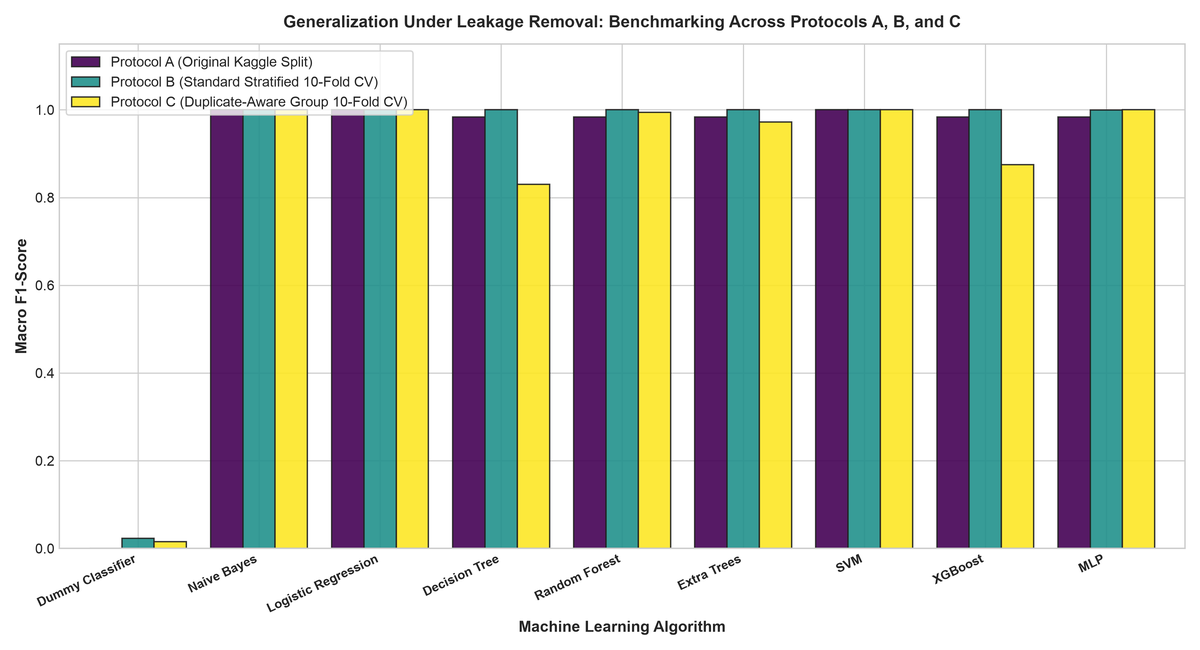
\includegraphics[width=0.9\textwidth]{protocol_comparison.png}
\caption{Cross-protocol performance comparison across the 9-model hierarchy. Notice the sharp degradation of Decision Tree and XGBoost under Protocol C.}
\label{fig:protocol_comparison}
\end{figure}

\begin{figure}[H]
\centering
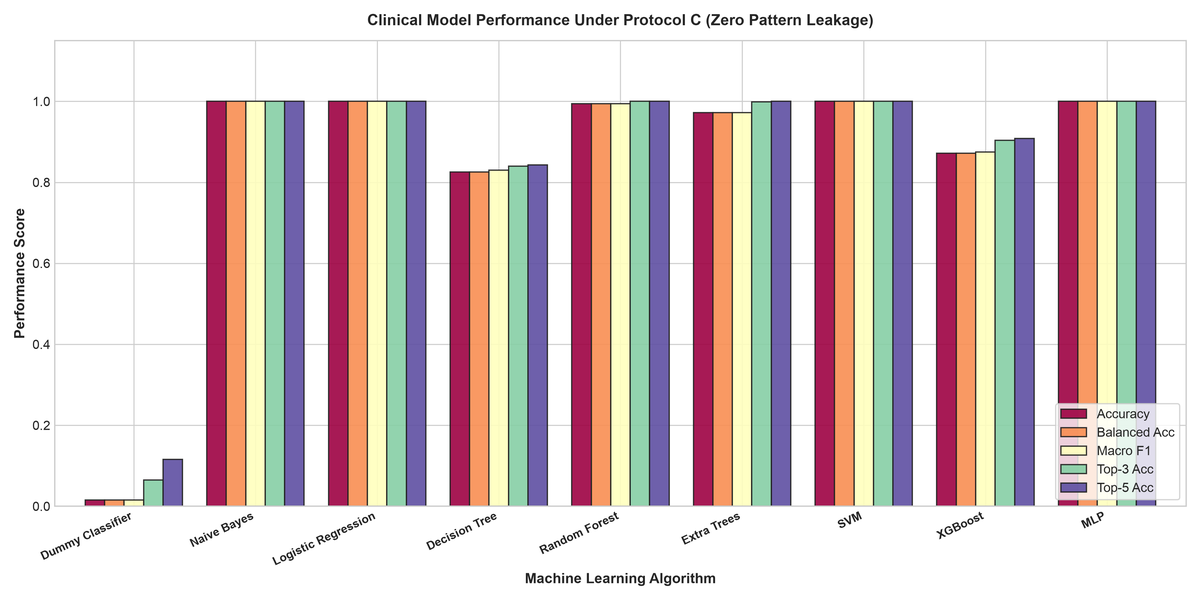
\includegraphics[width=0.9\textwidth]{model_performance.png}
\caption{Comprehensive metric breakdown under Protocol C (Zero Pattern Leakage), comparing Accuracy, Balanced Accuracy, Macro F1, Top-3, and Top-5 Accuracy.}
\label{fig:model_performance}
\end{figure}

% ==============================================================================
\section{Leakage-Aware Feature Selection and Dimensionality Reduction}
\label{sec:feature_selection}

To investigate whether multi-disease prediction requires all 132 symptoms or can operate on a compact clinical subset, we evaluated five feature-selection paradigms: Filter methods (Mutual Information, Chi-Square), Embedded methods ($L_1$-regularized Logistic Regression, Random Forest Gini importance), and Wrapper methods (Recursive Feature Elimination, RFE). Crucially, all feature ranking and selection procedures were fitted \emph{strictly inside each training fold} under Protocol C to prevent validation contamination.

\begin{table}[H]
\caption{Predictive Performance Across Feature Subsets ($k \in \{132, 100, 75, 50, 30, 20, 10\}$) Under Protocol C Across Model Families}
\label{tab:feature_selection_summary}
\centering
\scriptsize
\setlength{\tabcolsep}{2pt}
\begin{tabular}{cc|cccc|cccc|cccc}
\toprule
\multirow{2}{*}{\textbf{Method}} & \multirow{2}{*}{\textbf{$k$}} & \multicolumn{4}{c|}{\textbf{Logistic Regression}} & \multicolumn{4}{c|}{\textbf{MLP Neural Net}} & \multicolumn{4}{c}{\textbf{Random Forest}} \\
\cmidrule{3-14}
& & \textbf{Acc} & \textbf{F1} & \textbf{Top-3} & \textbf{Ret.} & \textbf{Acc} & \textbf{F1} & \textbf{Top-3} & \textbf{Ret.} & \textbf{Acc} & \textbf{F1} & \textbf{Top-3} & \textbf{Ret.} \\
\midrule
Full Baseline & 132 & 1.0000 & 1.0000 & 1.0000 & 100.0\% & 1.0000 & 1.0000 & 1.0000 & 100.0\% & 0.9939 & 0.9939 & 1.0000 & 100.0\% \\
\midrule
\multirow{6}{*}{Mutual Info}
& 100 & 0.9988 & 0.9988 & 1.0000 & 99.9\% & 0.9756 & 0.9765 & 0.9988 & 97.7\% & 0.9854 & 0.9854 & 0.9988 & 99.1\% \\
& 75  & 0.9939 & 0.9939 & 0.9988 & 99.4\% & 0.9610 & 0.9615 & 0.9976 & 96.2\% & 0.9817 & 0.9819 & 0.9988 & 98.8\% \\
& 50  & 0.9683 & 0.9687 & 0.9866 & \textbf{96.9\%}* & 0.9768 & 0.9773 & 0.9878 & \textbf{97.7\%}* & 0.9463 & 0.9471 & 0.9805 & \textbf{95.3\%}* \\
& 30  & 0.8354 & 0.8349 & 0.9585 & 83.5\% & 0.8415 & 0.8449 & 0.9476 & 84.5\% & 0.8098 & 0.8112 & 0.9512 & 81.6\% \\
& 20  & 0.7512 & 0.7520 & 0.9134 & 75.2\% & 0.7573 & 0.7567 & 0.9146 & 75.7\% & 0.7220 & 0.7237 & 0.8902 & 72.8\% \\
& 10  & 0.4329 & 0.4328 & 0.6707 & 43.3\% & 0.4415 & 0.4393 & 0.6585 & 43.9\% & 0.4329 & 0.4326 & 0.6500 & 43.5\% \\
\midrule
\multirow{6}{*}{$L_1$ Logistic}
& 100 & 0.9988 & 0.9988 & 1.0000 & 99.9\% & 0.9988 & 0.9988 & 1.0000 & 99.9\% & 0.9866 & 0.9866 & 1.0000 & 99.3\% \\
& 75  & 0.9939 & 0.9939 & 1.0000 & 99.4\% & 0.9829 & 0.9811 & 1.0000 & \textbf{98.1\%}* & 0.9793 & 0.9792 & 1.0000 & \textbf{98.5\%}* \\
& 50  & 0.9671 & 0.9671 & 0.9951 & \textbf{96.7\%}* & 0.9695 & 0.9702 & 0.9976 & \textbf{97.0\%}* & 0.9256 & 0.9263 & 0.9744 & 93.2\% \\
& 30  & 0.9110 & 0.9104 & 0.9805 & 91.0\% & 0.9293 & 0.9275 & 0.9866 & 92.8\% & 0.8915 & 0.8915 & 0.9659 & 89.7\% \\
& 20  & 0.8305 & 0.8313 & 0.9707 & 83.1\% & 0.8329 & 0.8438 & 0.9732 & 84.4\% & 0.8049 & 0.8052 & 0.9549 & 81.0\% \\
& 10  & 0.5280 & 0.5289 & 0.7976 & 52.9\% & 0.5317 & 0.5275 & 0.7768 & 52.8\% & 0.5098 & 0.5103 & 0.7610 & 51.3\% \\
\bottomrule
\end{tabular}
\vspace{2pt}
\par\noindent{\footnotesize *Meets the predefined operational retention criterion of $\ge 95.0\%$ retained Macro F1 relative to the 132-feature baseline. Ret. denotes Retained Macro-F1 percentage.}
\end{table}

\subsection{Smallest Subset Satisfying the \texorpdfstring{$\ge 95\%$}{>= 95\%} Retained Criterion}
\label{subsec:smallest_subset}
As documented in Table~\ref{tab:feature_selection_summary} and \cref{fig:feature_count_vs_f1}:
\begin{enumerate}
    \item Under both \textbf{Mutual Information} and \textbf{$L_1$ Logistic Regression}, \textbf{$k = 50$ symptoms} is the smallest feature subset that satisfies the predefined operational criterion of $\ge 95\%$ retained Macro-F1:
    \begin{itemize}
        \item Logistic Regression achieves \textbf{96.9\% retained F1} (F1: 0.9687, Top-3: 98.66\%) with Mutual Information.
        \item Multi-Layer Perceptron (MLP) achieves \textbf{97.7\% retained F1} (F1: 0.9773, Top-3: 98.78\%) with Mutual Information.
        \item Random Forest achieves \textbf{95.3\% retained F1} (F1: 0.9471, Top-3: 98.05\%) with Mutual Information.
    \end{itemize}
    \item We emphasize that the $\ge 95\%$ retained threshold is an \emph{operational benchmark threshold} defined for comparative evaluation, not clinical proof of exhaustive medical coverage.
\end{enumerate}

\begin{figure}[H]
\centering
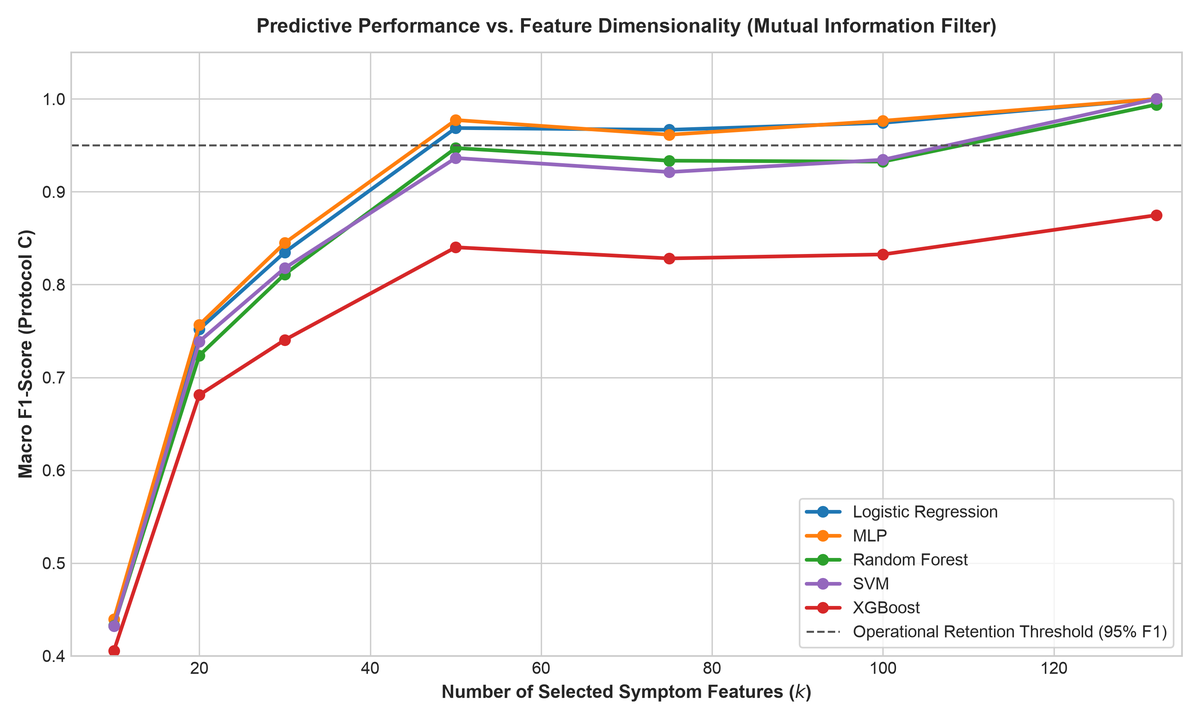
\includegraphics[width=0.9\textwidth]{feature_count_vs_macro_f1.png}
\caption{Macro F1-score as a function of symptom subset size ($k$) across models under Mutual Information feature selection. The dashed line marks the 95\% operational retention threshold.}
\label{fig:feature_count_vs_f1}
\end{figure}

\begin{figure}[H]
\centering
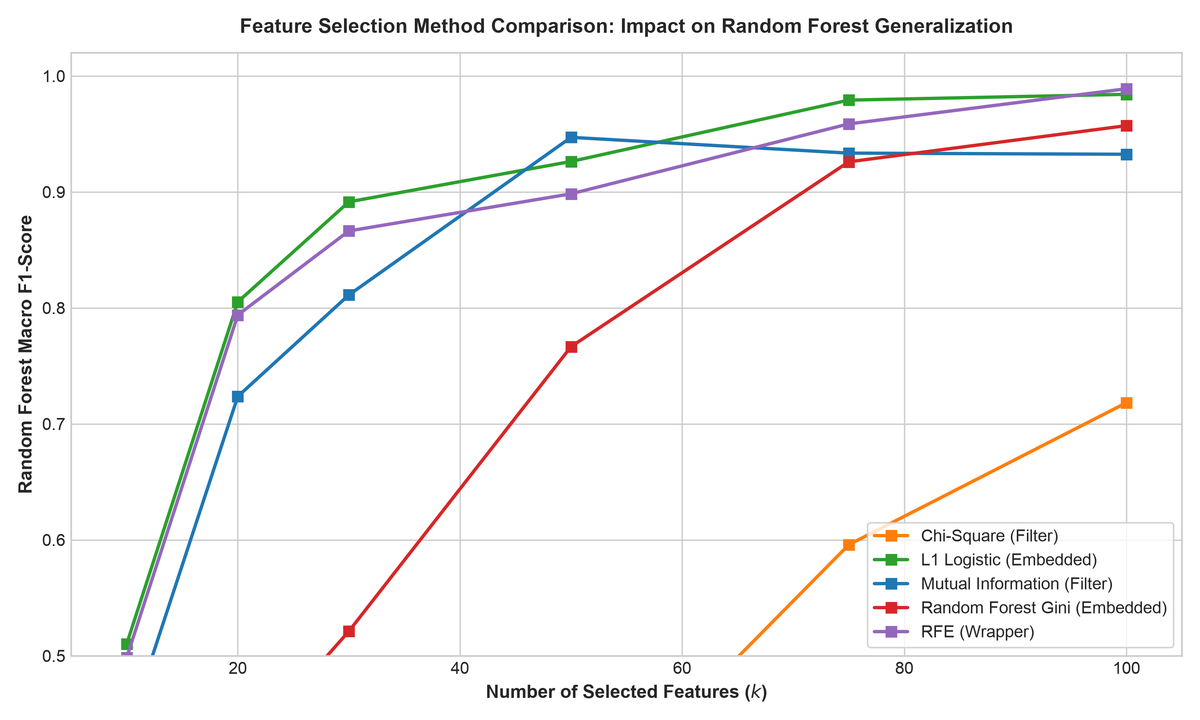
\includegraphics[width=0.9\textwidth]{feature_selection_comparison.png}
\caption{Feature selection method comparison on Random Forest under Protocol C. Notice the severe performance degradation of Chi-Square due to the suppression of high-information shared symptoms across overlapping diseases.}
\label{fig:feature_selection_comparison}
\end{figure}

\begin{figure}[H]
\centering
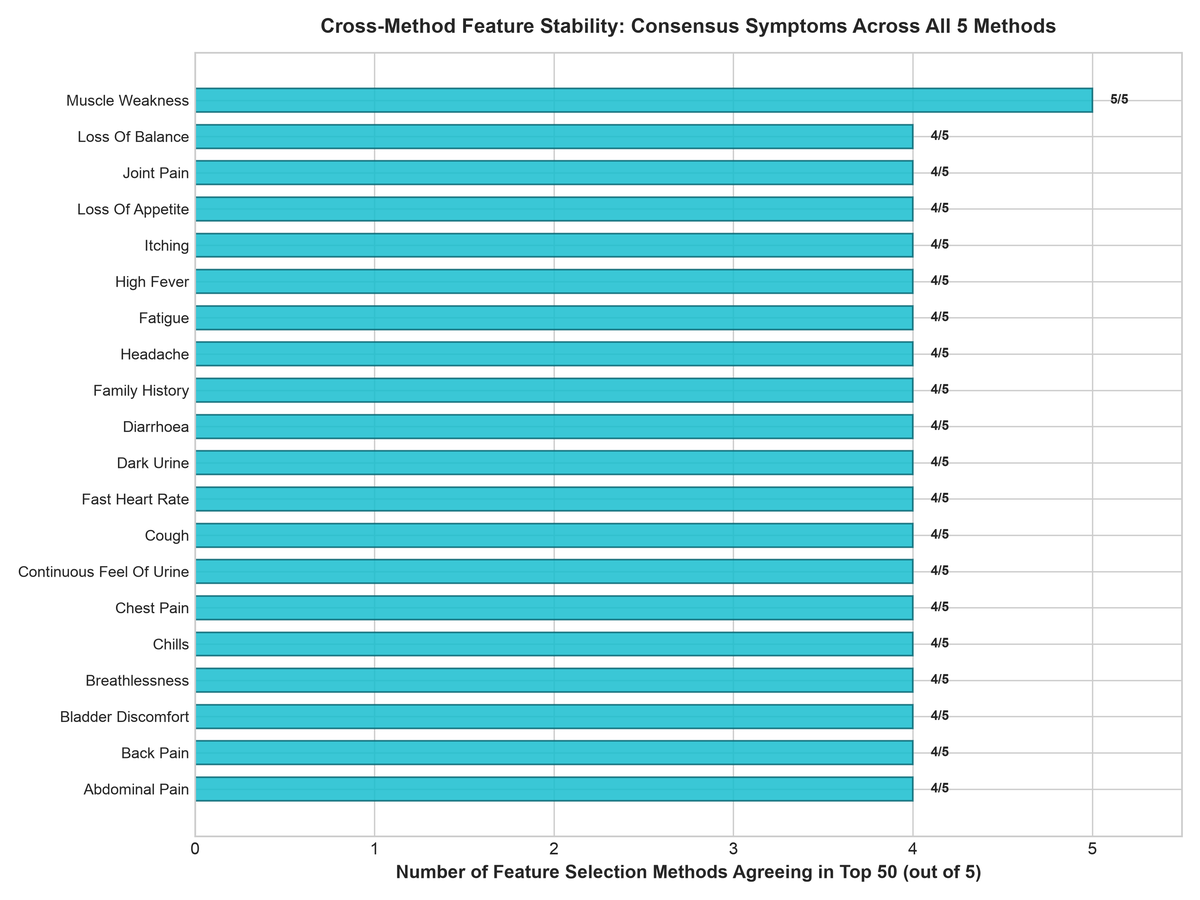
\includegraphics[width=0.9\textwidth]{feature_selection_stability.png}
\caption{Cross-method consensus: Top 20 symptoms identified consistently across independent feature selection methods within the top 50 ranked features.}
\label{fig:feature_selection_stability}
\end{figure}

\subsection{Differential Diagnosis Resilience at Aggressive Compression}
\label{subsec:differential_resilience}
When symptom dimensionality is aggressively reduced below $k=50$:
\begin{itemize}
    \item Under $L_1$ Logistic feature selection at \textbf{$k=30$ symptoms}, Top-1 Macro F1 declines to 0.9104, yet \textbf{Top-3 accuracy remains at 98.05\%} and \textbf{Top-5 accuracy reaches 99.02\%}.
    \item Even at \textbf{$k=20$ symptoms}, Top-3 accuracy is maintained at \textbf{97.07\%} and Top-5 accuracy at \textbf{98.29\%}.
    \item These results indicate that Top-$k$ evaluation can preserve substantially higher candidate-ranking performance than Top-1 classification under aggressive feature reduction.
\end{itemize}

\subsection{Empirical Analysis of Chi-Square Ranking Behavior}
\label{subsec:chisquare_analysis}
Under the duplicate-aware evaluation and feature-selection protocol used in this study, chi-square-based ranking produced substantially poorer predictive performance (declining to 71.4\% at $k=100$ and 35.4\% at $k=50$; \cref{fig:feature_selection_comparison}). A dataset-level audit revealed its ranking was strongly associated with symptom frequency and disease breadth ($r = -0.9069$ between $\chi^2$ score and prevalence):
\begin{enumerate}
    \item In a balanced 41-class cohort, binary symptoms occurring in only one disease achieve the maximum theoretical $\chi^2$ score ($\chi^2 = 4800.0$), ranking ultra-specific single-disease symptoms at the very top (20 symptoms covering only 9 of the 41 diseases).
    \item Conversely, high-information shared symptoms present across multiple conditions (e.g., \emph{vomiting} in 17 diseases, \emph{fatigue} in 17 diseases) received the lowest $\chi^2$ scores ($\chi^2 \approx 2704$).
    \item Because 32 of the 41 diseases lack exclusive private symptoms and depend primarily on combinations of shared symptoms, chi-square ranking stripped the models of the combinatorial features required to differentiate overlapping pathologies.
\end{enumerate}

\subsection{Feature Selection Stability Across Independent Folds}
\label{subsec:stability_folds}
To verify that the $k=50$ threshold does not reflect an artifact of a single lucky split, we audited selection stability across all 10 independent duplicate-aware folds:
\begin{itemize}
    \item For Mutual Information, the top 15 features exhibited \textbf{10/10 selection stability} across all 10 folds: \emph{fatigue, vomiting, high fever, loss of appetite, nausea, headache, abdominal pain, yellowish skin, yellowing of eyes, chills, skin rash, malaise, chest pain, joint pain,} and \emph{sweating}.
    \item For $L_1$ Logistic Regression, 15 symptoms also achieved 10/10 fold stability.
    \item Across all five independent feature-selection paradigms, 31 symptoms achieved $\ge 80\%$ cross-method consensus (\cref{fig:feature_selection_stability}), confirming that the compressed feature space captures clinically established core diagnostic indicators.
\end{itemize}


% CHAPTER VI: Clinical Robustness and Sparsity Analysis
\chapter{Clinical Symptom Sparsity and Cold-Start Robustness}
\label{chap:sparsity}

While feature selection (\cref{chap:results_feature_selection}) identifies a compact global ontology for model construction, real-world deployment requires robustness against incomplete symptom presentation. When an intake profile presents only a restricted subset of chief symptoms ($s \in [1, 10]$ active symptoms) rather than an exhaustive symptom profile (cohort natural mean: $7.45 \pm 3.59$ active symptoms, range 3--17), models must degrade gracefully. In this chapter, we evaluate this behavior through controlled stochastic masking experiments under Protocol C. 

\begin{figure}[H]
\centering
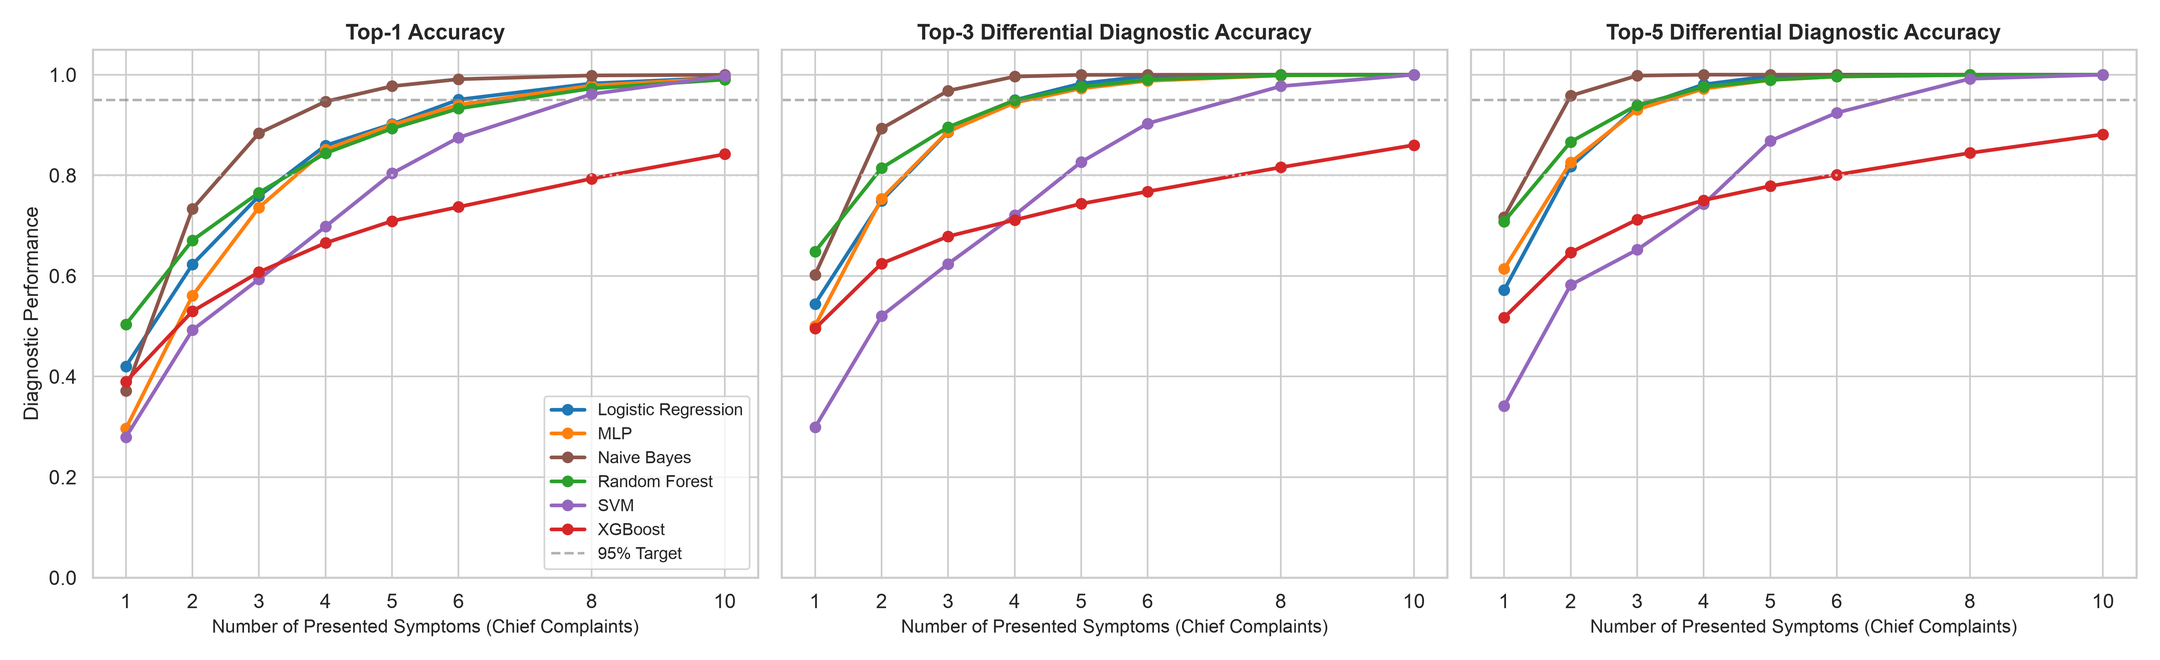
\includegraphics[width=\textwidth]{sparsity_decay_curves.png}
\caption{Diagnostic performance degradation curves under simulated patient intake sparsity ($s \in [1, 10]$ presenting chief complaints) across six model architectures evaluated under Protocol C. Left: Top-1 single-label accuracy. Centre: Top-3 differential diagnostic accuracy. Right: Top-5 differential diagnostic accuracy. The horizontal dashed line marks the 95\% operational retention threshold. \textit{Note: Curves reflect provisional Phase 5 benchmark outputs across available masking seeds; final parameter freezing awaits completed seed matrix execution.}}
\label{fig:sparsity_decay_curves}
\end{figure}

\section{Experimental Design and Stochastic Sparsity Protocol}
\label{sec:sparsity_design}
To evaluate model resilience under controlled symptom restriction on this benchmark, models were evaluated under Protocol C across restricted symptom budgets $s \in \{\text{Full}, 10, 8, 6, 5, 4, 3, 2, 1\}$ using five independent random seeds applied across all test records. For each test sample presenting $P$ positive symptoms, if $P > s$, exactly $s$ positive symptoms were selected uniformly at random while remaining symptoms were masked to zero; if $P \le s$, the sample remained unmasked. Evaluations were conducted across both the Full 132-symptom space and the Frozen 50-symptom space identified in Phase 4.

Crucially, these controlled masking experiments represent a benchmark-specific synthetic stress test designed to quantify how algorithmic architectures respond to incomplete binary feature vectors on this dataset; they do not establish clinical diagnostic efficacy in real-world patient encounters. Furthermore, the experimental outputs reported in this chapter are \textbf{provisional}, reflecting the currently available Phase 5 runs across available masking seeds. 

\begin{table}[H]
\caption{Provisional Diagnostic Resilience Under Simulated Symptom Sparsity on the Kaggle Benchmark (Protocol C, Across Available Masking Seeds)}
\label{tab:sparsity_summary}
\centering
\scriptsize
\setlength{\tabcolsep}{3pt}
\begin{tabular}{cc|cccc|cccc}
\toprule
\multirow{2}{*}{\textbf{Model}} & \multirow{2}{*}{\textbf{Budget ($s$)}} & \multicolumn{4}{c|}{\textbf{Full 132-Symptom Space}} & \multicolumn{4}{c}{\textbf{Frozen 50-Symptom Space}} \\
\cmidrule{3-10}
& & \textbf{Top-1 Acc} & \textbf{Macro-F1} & \textbf{Top-3 Acc} & \textbf{Top-5 Acc} & \textbf{Top-1 Acc} & \textbf{Macro-F1} & \textbf{Top-3 Acc} & \textbf{Top-5 Acc} \\
\midrule
\multirow{5}{*}{Log. Reg.}
& Full (7.45$\pm$3.59) & $1.000 \pm 0.000$ & $1.000 \pm 0.000$ & 1.000 & 1.000 & $0.961 \pm 0.029$ & $0.895 \pm 0.065$ & 0.987 & 0.995 \\
& 8 Symptoms  & $0.983 \pm 0.017$ & $0.960 \pm 0.035$ & 1.000 & 1.000 & $0.942 \pm 0.028$ & $0.845 \pm 0.057$ & 0.987 & 0.995 \\
& 5 Symptoms  & $0.902 \pm 0.054$ & $0.775 \pm 0.054$ & 0.983 & 0.997 & $0.755 \pm 0.066$ & $0.546 \pm 0.054$ & 0.930 & 0.976 \\
& 3 Symptoms  & $0.759 \pm 0.076$ & $0.553 \pm 0.049$ & 0.886 & 0.936 & $0.533 \pm 0.130$ & $0.284 \pm 0.063$ & 0.743 & 0.873 \\
& 1 Symptom   & $0.420 \pm 0.089$ & $0.235 \pm 0.039$ & 0.544 & 0.572 & $0.187 \pm 0.105$ & $0.070 \pm 0.028$ & 0.406 & 0.480 \\
\midrule
\multirow{5}{*}{Rand. Forest}
& Full (7.45$\pm$3.59) & $0.994 \pm 0.010$ & $0.987 \pm 0.022$ & 1.000 & 1.000 & $0.940 \pm 0.027$ & $0.844 \pm 0.057$ & 0.982 & 0.982 \\
& 8 Symptoms  & $0.973 \pm 0.018$ & $0.932 \pm 0.039$ & 0.999 & 0.999 & $0.922 \pm 0.032$ & $0.797 \pm 0.049$ & 0.975 & 0.976 \\
& 5 Symptoms  & $0.893 \pm 0.058$ & $0.771 \pm 0.070$ & 0.976 & 0.990 & $0.818 \pm 0.058$ & $0.598 \pm 0.058$ & 0.941 & 0.960 \\
& 3 Symptoms  & $0.765 \pm 0.092$ & $0.571 \pm 0.062$ & 0.896 & 0.940 & $0.584 \pm 0.116$ & $0.330 \pm 0.050$ & 0.833 & 0.912 \\
& 1 Symptom   & $0.504 \pm 0.087$ & $0.310 \pm 0.046$ & 0.648 & 0.708 & $0.240 \pm 0.127$ & $0.096 \pm 0.040$ & 0.556 & 0.629 \\
\midrule
\multirow{5}{*}{SVM (RBF)}
& Full (7.45$\pm$3.59) & $1.000 \pm 0.000$ & $1.000 \pm 0.000$ & 1.000 & 1.000 & $0.939 \pm 0.031$ & $0.844 \pm 0.069$ & 0.963 & 0.970 \\
& 8 Symptoms  & $0.961 \pm 0.029$ & $0.904 \pm 0.051$ & 0.977 & 0.992 & $0.920 \pm 0.038$ & $0.803 \pm 0.068$ & 0.956 & 0.968 \\
& 5 Symptoms  & $0.804 \pm 0.087$ & $0.618 \pm 0.045$ & 0.826 & 0.868 & $0.769 \pm 0.054$ & $0.517 \pm 0.054$ & 0.809 & 0.873 \\
& 3 Symptoms  & $0.593 \pm 0.112$ & $0.374 \pm 0.056$ & 0.624 & 0.652 & $0.523 \pm 0.132$ & $0.260 \pm 0.055$ & 0.548 & 0.601 \\
& 1 Symptom   & $0.279 \pm 0.123$ & $0.150 \pm 0.046$ & 0.299 & 0.341 & $0.206 \pm 0.125$ & $0.079 \pm 0.032$ & 0.253 & 0.331 \\
\midrule
\multirow{5}{*}{MLP}
& Full (7.45$\pm$3.59) & $1.000 \pm 0.000$ & $1.000 \pm 0.000$ & 1.000 & 1.000 & $0.977 \pm 0.024$ & $0.934 \pm 0.057$ & 0.990 & 1.000 \\
& 8 Symptoms  & $0.978 \pm 0.018$ & $0.952 \pm 0.040$ & 0.999 & 1.000 & $0.957 \pm 0.029$ & $0.883 \pm 0.054$ & 0.990 & 1.000 \\
& 5 Symptoms  & $0.900 \pm 0.049$ & $0.792 \pm 0.066$ & 0.973 & 0.989 & $0.836 \pm 0.053$ & $0.647 \pm 0.040$ & 0.948 & 0.986 \\
& 3 Symptoms  & $0.736 \pm 0.106$ & $0.580 \pm 0.065$ & 0.887 & 0.931 & $0.618 \pm 0.086$ & $0.385 \pm 0.041$ & 0.811 & 0.893 \\
& 1 Symptom   & $0.296 \pm 0.119$ & $0.215 \pm 0.041$ & 0.500 & 0.614 & $0.206 \pm 0.107$ & $0.090 \pm 0.033$ & 0.439 & 0.519 \\
\midrule
\multirow{5}{*}{XGBoost}
& Full (7.45$\pm$3.59) & $0.884 \pm 0.045$ & $0.680 \pm 0.109$ & 0.903 & 0.920 & $0.854 \pm 0.037$ & $0.580 \pm 0.078$ & 0.909 & 0.924 \\
& 8 Symptoms  & $0.793 \pm 0.045$ & $0.547 \pm 0.086$ & 0.816 & 0.844 & $0.777 \pm 0.045$ & $0.471 \pm 0.067$ & 0.844 & 0.875 \\
& 5 Symptoms  & $0.709 \pm 0.055$ & $0.435 \pm 0.065$ & 0.743 & 0.779 & $0.634 \pm 0.103$ & $0.326 \pm 0.072$ & 0.722 & 0.774 \\
& 3 Symptoms  & $0.607 \pm 0.063$ & $0.339 \pm 0.055$ & 0.679 & 0.712 & $0.509 \pm 0.116$ & $0.229 \pm 0.066$ & 0.621 & 0.676 \\
& 1 Symptom   & $0.390 \pm 0.077$ & $0.209 \pm 0.040$ & 0.495 & 0.517 & $0.217 \pm 0.111$ & $0.091 \pm 0.031$ & 0.373 & 0.487 \\
\midrule
\multirow{5}{*}{Naive Bayes}
& Full (7.45$\pm$3.59) & $1.000 \pm 0.000$ & $1.000 \pm 0.000$ & 1.000 & 1.000 & $0.864 \pm 0.094$ & $0.883 \pm 0.082$ & 0.965 & 0.972 \\
& 8 Symptoms  & $0.999 \pm 0.004$ & $0.998 \pm 0.004$ & 1.000 & 1.000 & $0.859 \pm 0.085$ & $0.877 \pm 0.075$ & 0.965 & 0.972 \\
& 5 Symptoms  & $0.977 \pm 0.022$ & $0.969 \pm 0.023$ & 1.000 & 1.000 & $0.832 \pm 0.084$ & $0.834 \pm 0.073$ & 0.964 & 0.972 \\
& 3 Symptoms  & $0.884 \pm 0.053$ & $0.829 \pm 0.043$ & 0.968 & 0.998 & $0.722 \pm 0.077$ & $0.667 \pm 0.060$ & 0.926 & 0.970 \\
& 1 Symptom   & $0.372 \pm 0.081$ & $0.313 \pm 0.033$ & 0.602 & 0.717 & $0.145 \pm 0.047$ & $0.137 \pm 0.020$ & 0.489 & 0.658 \\
\bottomrule
\end{tabular}
\begin{flushleft}
\scriptsize
\textit{Note: Results report mean $\pm$ standard deviation across evaluated masking seeds. These values are provisional pending complete model-by-budget-by-seed matrix completion. Baseline full-input OOF Macro-F1 scores exhibit variations across specific cross-validation splits and model configurations (e.g., Random Forest: 0.9866--0.9963; MLP: 0.9803--1.0000; SVM: 0.9915--1.0000; XGBoost: 0.6802--0.9137). Neither Table~\ref{tab:sparsity_summary} nor Figure~\ref{fig:sparsity_decay_curves} should be regarded as frozen parameters prior to final experimental reconciliation.}
\end{flushleft}
\end{table}

\section{The Differential Diagnostic Safeguard Under Sparsity}
\label{sec:differential_safeguard}
As documented in Table~\ref{tab:sparsity_summary} and \cref{fig:sparsity_decay_curves}, progressive symptom restriction induces two contrasting empirical regimes across the evaluated models:
\begin{enumerate}
    \item \textbf{Single-Label Accuracy Collapse}: Top-1 accuracy experiences a steep decline as presenting symptoms fall below $s = 5$. At $s = 3$ presenting symptoms (simulating acute reporting restriction), Top-1 accuracy declines to 75.9\% (Macro-F1: 55.3\%) for Logistic Regression, 76.5\% (Macro-F1: 57.1\%) for Random Forest, and 73.6\% (Macro-F1: 58.0\%) for MLP on the Full 132 space. At $s = 1$, Top-1 accuracy falls into the 27.9\%--50.4\% range (Macro-F1: 15.0\%--31.3\%) across all models.
    \item \textbf{Differential Diagnostic Buffer}: In sharp contrast, multi-candidate ranking demonstrates remarkable resilience. At $s = 3$ symptoms, \textbf{Top-3 diagnostic accuracy remains above 88.6\%} for Logistic Regression (88.6\%), Random Forest (89.6\%), and MLP (88.7\%), with Naive Bayes reaching 96.8\%, while \textbf{Top-5 accuracy exceeds 93.0\%} across these architectures. Even at $s = 2$ presenting symptoms, Top-5 inclusion remains between 81.7\% and 86.7\% for the leading models.
\end{enumerate}

These empirical observations highlight the vital safeguard provided by differential candidate ranking over rigid single-label classification under simulated sparsity: presenting an ordered candidate list (Top-3 to Top-5) ensures that the true disease label is captured in over 93\% of evaluated cases under moderate symptom restriction on this benchmark, providing a candidate buffer prior to confirmatory diagnostics.

\section{Architectural Sensitivity and Representation Resilience}
\label{sec:arch_sensitivity}
\begin{itemize}
    \item \textbf{Additive vs.\ Partitioning Models}: Linear (Logistic Regression) and neural (MLP) architectures degrade gracefully under moderate sparsity ($s \ge 4$), as their additive decision boundaries aggregate evidence from whatever subset of features is present. Tree ensembles (Random Forest, XGBoost) experience steeper drops when higher-level tree split nodes interrogate features that the patient omitted, though Random Forest maintains higher Top-1 retention at extreme sparsity ($s=1$, 50.4\%) due to bootstrap feature subsampling.
    \item \textbf{Kernel and Probabilistic Baselines}: SVM (RBF) degrades sharply at $s \le 3$ (Top-1 59.3\% at $s=3$ and 27.9\% at $s=1$) because geometric distances in the 132-dimensional kernel space are distorted by large fractions of zeroed dimensions. Conversely, Naive Bayes retains exceptionally high Top-3 and Top-5 candidate retention under moderate sparsity ($s=5$, Top-3 100.0\%), though its single-label accuracy collapses at $s=1$ (37.2\%).
    \item \textbf{Representation Generalization (132 vs.\ 50 Features)}: Evaluating models trained on the Frozen 50-symptom space revealed that retaining only core consensus features achieves comparable sparsity decay trajectories to the uncompressed 132-symptom model down to $s=5$. Below $s=4$, the reduced feature pool accelerates degradation because masking active symptoms leaves fewer alternative informative features within the 50-symptom subspace.
\end{itemize}

In summary, the degradation profiles underscore that candidate differential ranking mitigates information loss when symptom reporting is incomplete. However, final confirmation of these trajectories requires the ongoing full seed-by-budget re-run and ultimate validation against real-world clinical patient registries.


% CHAPTER VII: Discussion, Conclusion and Future Work
\chapter{Discussion, Conclusion, and Future Work}
\label{chap:conclusion}

\section{Discussion and Limitations}
\label{sec:discussion}

\subsection{Scientific Limitations}
\label{subsec:scientific_limitations}
The Kaggle Disease Prediction dataset is a rule-derived benchmark rather than a prospective clinical patient cohort. The absence of patient demographics (age, sex, vitals, medical history, comorbidities) represents an inherent structural constraint. Consequently, this system is strictly evaluated as an algorithmic decision-support prototype under simulated benchmark stress testing. Statistical stability across feature selection algorithms and cross-validation folds establishes dataset-level algorithmic evidence, but does not substitute for independent external clinical validation.

\subsection{Ethical Framework and Clinical Safety}
\label{subsec:ethical_framework}
The decision-support prototype is engineered with explicit safety constraints: it outputs candidate probabilities, supporting/opposing evidence, and a mandatory disclaimer advising formal clinical consultation. The system is explicitly designed as an assistive triage aid, not an autonomous diagnostic agent.

\section{Conclusion}
\label{sec:conclusion}

This research establishes a rigorous, leakage-aware foundation for symptom-based disease prediction:
\begin{enumerate}
    \item By forensically exposing the 93.8\% synthetic duplication and 97.6\% train-test leakage in the widely cited Kaggle benchmark, we demonstrate why prevailing na\"{i}ve 100\% accuracy claims are methodologically flawed.
    \item Through leakage-aware Duplicate-Aware Group Cross-Validation (Protocol C), we proved that partitioned tree-based models suffer substantial degradation (Decision Tree: $-17.44\%$, XGBoost: $-12.80\%$) when evaluated on genuinely unseen symptom profiles, confirming Hypothesis H1.
    \item Our leakage-aware feature selection demonstrates that a compact set of 50 consensus symptoms preserves $\ge 95\%$ retained Macro-F1 on the benchmark, identifying an algorithmically stable symptom ontology without sacrificing core predictive fidelity.
    \item Under controlled symptom sparsity simulations, we observed that while single-label Top-1 accuracy declines steeply as inputs are restricted to acute chief complaints ($s \le 3$), Top-3 and Top-5 candidate ranking retains over 88\% and 93\% inclusion on this benchmark. This provisional finding highlights the critical buffer provided by differential candidate ranking when patient intake profiles are incomplete.
\end{enumerate}

\section{Key Findings Summary}
\label{sec:key_findings}
\begin{itemize}
    \item The Kaggle Disease Prediction dataset contains only 304 unique symptom vectors across 4,920 training records (93.8\% duplication), with 41 of 42 test records being verbatim duplicates of training records.
    \item Duplicate-Aware Group CV (Protocol C) exposes that Decision Tree accuracy collapses by $-17.44\%$ and XGBoost by $-12.80\%$ relative to standard cross-validation.
    \item A compact ontology of 50 consensus symptoms satisfies the $\ge 95\%$ retained Macro-F1 operational criterion at the dataset level, establishing algorithmic feature stability on this benchmark.
    \item Multi-candidate differential ranking (Top-3 and Top-5) consistently provides a resilient safeguard against single-label accuracy collapse under both feature reduction and simulated symptom sparsity.
\end{itemize}

\section{Future Work and Research Roadmap}
\label{sec:future_work}

The findings of this thesis provide an empirical baseline for several immediate research extensions:

\subsection{Reconciliation of Complete Sparsity Matrix}
\label{subsec:sparsity_reconciliation}
The immediate priority is completing the full model-by-budget-by-seed experimental matrix for Phase 5 across all five random seeds, reconciling baseline cross-validation variances across all six model families, and freezing the final empirical degradation parameters.

\subsection{Noise Robustness and Asymmetry Profiling (Hypothesis H3)}
\label{subsec:noise_robustness}
Building upon the sparsity stress test, Phase 6 will systematically profile model degradation under stochastic reporting noise, testing the hypothesis that false-positive symptom activations cause steeper performance drops than false-negative symptom dropouts across error rates up to 30\%.

\subsection{Probability Calibration and Uncertainty Quantification (Hypothesis H4)}
\label{subsec:calibration_roadmap}
Evaluating post-hoc calibration methods (Platt scaling, Isotonic regression, and temperature scaling) to minimize Expected Calibration Error (ECE) and Brier scores across neural and tree models, ensuring that output candidate probabilities accurately reflect diagnostic likelihoods.

\subsection{TreeSHAP Clinical Literature Concordance Audit (Hypothesis H5)}
\label{subsec:shap_audit}
Conducting an in-depth global and local feature attribution audit using TreeSHAP, systematically cross-referencing high-weight predictive symptoms against diagnostic criteria published by the World Health Organization (WHO) and the Centers for Disease Control and Prevention (CDC).

\subsection{Prospective Real-World Clinical Validation}
\label{subsec:real_world_validation}
Finally, validating the algorithmic framework on prospectively collected clinical patient cohorts featuring authentic demographic diversity, laboratory telemetry, and complex real-world comorbidities to evaluate generalizability beyond synthetic rule-derived benchmarks.


% Bibliography
\bibliographystyle{ieeetr}
\bibliography{references}

\end{document}
